{
\begin{figure*}[th]\normalsize
\begin{minipage}{3.2in}
\begin{center}
\begin{tabular}{ c | c | c | c | c | c }\normalsize
\normalsize Workload & \normalsize Read & \normalsize Update & \normalsize Scan & \normalsize Insert & \normalsize R\&U \\
\hline
A & 50\% & 50\% & - & - & - \\
B & 95\% & 5\% & - & - & - \\
C & 100\% & - & - & - & - \\
D & 95\% & - & - & 5\% & - \\
E & - & - & 95\% & 5\% & - \\
F & 50\% & - & - & - & 50\% \\
\end{tabular}
\end{center}
\vspace{-0.2in}
\mycaption{tbl-ycsb}{YCSB Workload Properties.}
{
The percentage of operations in each YCSB workload. 
R\&U stands for Read and Update.
}
\end{minipage}
\begin{minipage}{0.05in}
\hspace{0.05in}
\end{minipage}
\begin{minipage}{3.6in}
\begin{center}
\centerline{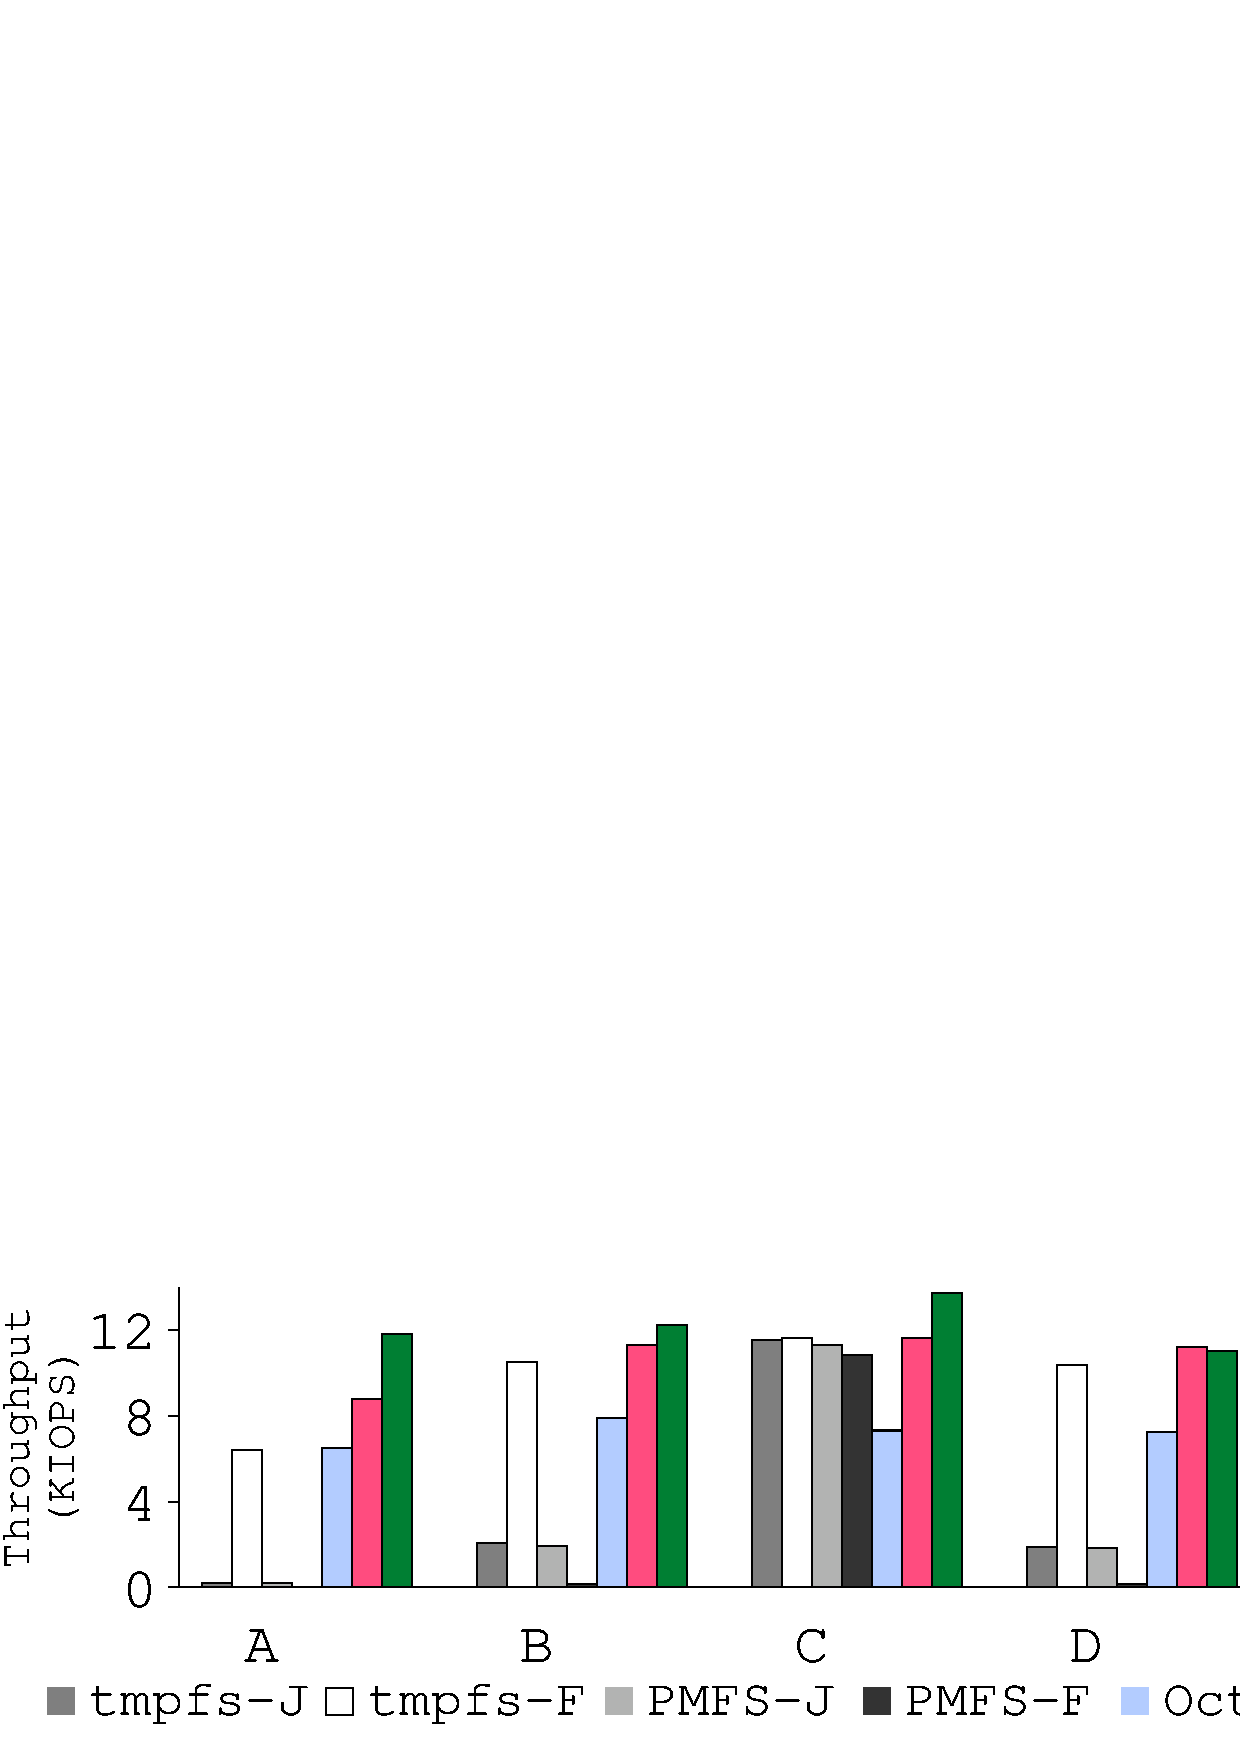
\includegraphics[width=3.8in]{Figures/g_plot_YCSB_run_throughput.pdf}}
\mycaption{fig-ycsbrun}{YCSB Workloads Throughput.}
{
}
\end{center}
\end{minipage}
\vspace{-0.2in}
\end{figure*}
}
